\section{Open-Vocabulary Segmentation}
\label{sec:open-vocabulary-segmentation}

The previous section established the dataset and metric coordinates used to evaluate open-vocabulary, promptable, grounded, and reasoning segmentation. This section reviews the first main technical route: open-vocabulary segmentation. Its central objective is to replace a fixed classifier head with a language-defined vocabulary while keeping dense spatial prediction reliable. In this setting, the input is usually an image and a set of category names or textual descriptions, and the output is a semantic, instance, or panoptic mask map whose labels may include unseen categories. Compared with the promptable and reasoning systems reviewed in later sections, open-vocabulary segmentation is less concerned with dialogue or implicit target inference; its core problem is the semantic-spatial transfer from vision-language foundation models to pixels, regions, and masks.

Existing work can be broadly grouped into four routes, as summarized in Table~\ref{tab:open-vocab-methods}. CLIP-based dense alignment directly turns image-text representations into pixel or patch classifiers. Proposal-then-classification methods first generate masks and then classify each mask with a text-defined recognition module. Fine-grained semantic methods enrich the label side or the segment side so that parts, attributes, and hierarchical concepts can be recognized. Efficiency, adaptation, and distillation methods focus on making open-vocabulary segmentation practical under limited labels, target-domain shifts, or training-free deployment. These routes are not mutually exclusive, but they expose different bottlenecks: dense alignment struggles with spatial localization, proposal pipelines depend on mask quality and mask-text calibration, fine-grained methods depend on data and name quality, and efficient methods often trade adaptability for stability.

\begin{table*}[t]
\centering
\small
\setlength{\tabcolsep}{5pt}
\renewcommand{\arraystretch}{1.34}
\caption{Representative open-vocabulary segmentation methods. The table is an index for Section~\ref{sec:open-vocabulary-segmentation}; detailed limitations are discussed in the corresponding subsections.}
\label{tab:open-vocab-methods}
\begin{tabularx}{\textwidth}{>{\raggedright\arraybackslash}p{0.17\textwidth}>{\raggedright\arraybackslash}X>{\raggedright\arraybackslash}p{0.24\textwidth}>{\raggedright\arraybackslash}p{0.28\textwidth}}
\toprule
Route & Representative methods & Foundation and setup & Key idea \\
\midrule
Mask-adapted region recognition & OVSeg~\citep{liang2023ovseg}; SAN~\citep{xu2023san}; Mask-Adapter~\citep{yliMaskadapterDevilMasks2025} & CLIP with MaskFormer, side adapters, or proposal masks; mask labels or caption-derived mask-category pairs & Adapts image-text representations to masked regions so that proposal-wise masks can be assigned open-vocabulary labels. \\
Open-vocabulary panoptic and diffusion-assisted parsing & ODISE~\citep{xu2023odise} and related diffusion or generative segmenters & Text-to-image diffusion models and CLIP-like classifiers; panoptic or segmentation training with prompts & Uses generative visual priors to extend open-vocabulary recognition from semantic masks to instance and panoptic parsing. \\
Universal segment embeddings & USE~\citep{xwangUseUniversalSegment2024}; ReME~\citep{xxuanReMEDataCentricFramework2025} & SAM or class-agnostic segmenters plus VLM/MLLM data engines; curated segment-text pairs or retrieval sets & Treats masks as reusable semantic units and aligns them with object, part, context, or descriptive language. \\
Patch and pixel-level CLIP alignment & PnP-OVSS~\citep{luo2024pnpovss}; DPSeg~\citep{zzhaoDPSegDualpromptCost2025}; dino.txt~\citep{joseDinov2MeetsText2025}; CLIP-Adapted Region-to-Text~\citep{gejCLIPAdaptedRegiontoTextLearning2025} & CLIP, BLIP-like VLMs, DINOv2, and visual prompts; training-free extraction, weak alignment, or cost-volume learning & Transfers language alignment to patches or pixels through attention, prompt interaction, cost volumes, or text-aligned dense backbones. \\
Training-free spatial enhancement & ITACLIP~\citep{maaydinItaclipBoostingTrainingfree2025}; CLIPer~\citep{lsunCliperHierarchicallyImproving2025}; CorrCLIP~\citep{dzhangCorrclipReconstructingPatch2025}; Trident~\citep{shiyHarnessingVisionFoundation2025} & CLIP with DINO, SAM, diffusion, or attention modification; no target training & Preserves CLIP generalization while repairing spatial coherence through attention rewriting, early-layer fusion, patch correlations, or VFM guidance. \\
Prompt, adapter, and test-time adaptation & Parameter-efficient hyperspherical tuning~\citep{zpengParameterefficientFinetuningHyperspherical2025}; semantic library adaptation~\citep{rqorbaniSemanticLibraryAdaptation2025}; MLMP TTA~\citep{noorimTesttimeAdaptationVisionlanguage2026} & CLIP or VLM segmentation backbones; few-shot, parameter-efficient, retrieval-based, or test-time adaptation & Improves deployment under limited labels or distribution shift without fully retraining the foundation model. \\
Benchmark and name refinement & RENOVATE~\citep{hhuangRenovatingNamesOpenvocabulary2024}; FLOSS~\citep{ybenigmimFlossFreeLunch2025}; similar semantic-space tests~\citep{yliuSteppingOutSimilar2025} & Foundation-model assisted data curation; benchmark renovation or protocol analysis & Shows that class names, synonyms, label granularity, and semantic-space choices can change measured open-vocabulary performance. \\
Domain-specific open vocabularies & OVRSIS/RSKT-Seg~\citep{libExploringEfficientOpenvocabulary2026}; AeroSeg~\citep{sduttaAerosegHarnessingSam2025}; ZoRI~\citep{huangZoRIDiscriminativeZeroshot2025}; RGB-thermal OVS~\citep{zhaoOpenvocabularyRGBThermalSemantic2024} & CLIP, SAM, remote-sensing priors, or multi-modal inputs; remote-sensing or cross-modal evaluation & Tests whether open-vocabulary segmentation transfers from natural-image benchmarks to domain-specific vocabularies and imaging conditions. \\
\bottomrule
\end{tabularx}
\end{table*}

\subsection{CLIP-based dense alignment}

CLIP-based dense alignment aims to convert image-level vision-language representations into spatially meaningful predictions. A direct rule compares each patch or pixel feature with text embeddings of the target vocabulary, but this naive transfer is weak because CLIP is trained to align whole images and captions rather than local regions and category masks. The resulting patch features may recognize the presence of an object while failing to preserve complete object extent, boundary details, or discriminability between adjacent categories. This is the basic semantic-spatial gap behind many open-vocabulary segmentation methods.

Early training-based methods address this gap by adapting CLIP or a CLIP-compatible segmentation network to dense prediction. OVSeg observes that two-stage pipelines are bottlenecked by CLIP classification on masked crops rather than by mask proposal quality, and therefore adapts CLIP with caption-derived mask-category pairs and mask prompt tuning~\citep{liang2023ovseg}. SAN instead attaches a lightweight side adapter to a frozen CLIP model, generating mask proposals and attention biases in a single end-to-end framework so that mask prediction becomes CLIP-aware~\citep{xu2023san}. Later dense alignment methods refine the pixel-text similarity map itself. DPSeg constructs dual-prompt cost volumes by combining text prompts with visual prompts, arguing that same-modality visual prompts can reduce the image-text embedding gap and provide sharper localization cues~\citep{zzhaoDPSegDualpromptCost2025}. dino.txt takes a different route: it aligns a text encoder with a frozen DINOv2 visual backbone so that strong self-supervised dense features acquire a language interface for both image-level and pixel-level recognition~\citep{joseDinov2MeetsText2025}.

\begin{figure}[htbp]
    \centering
    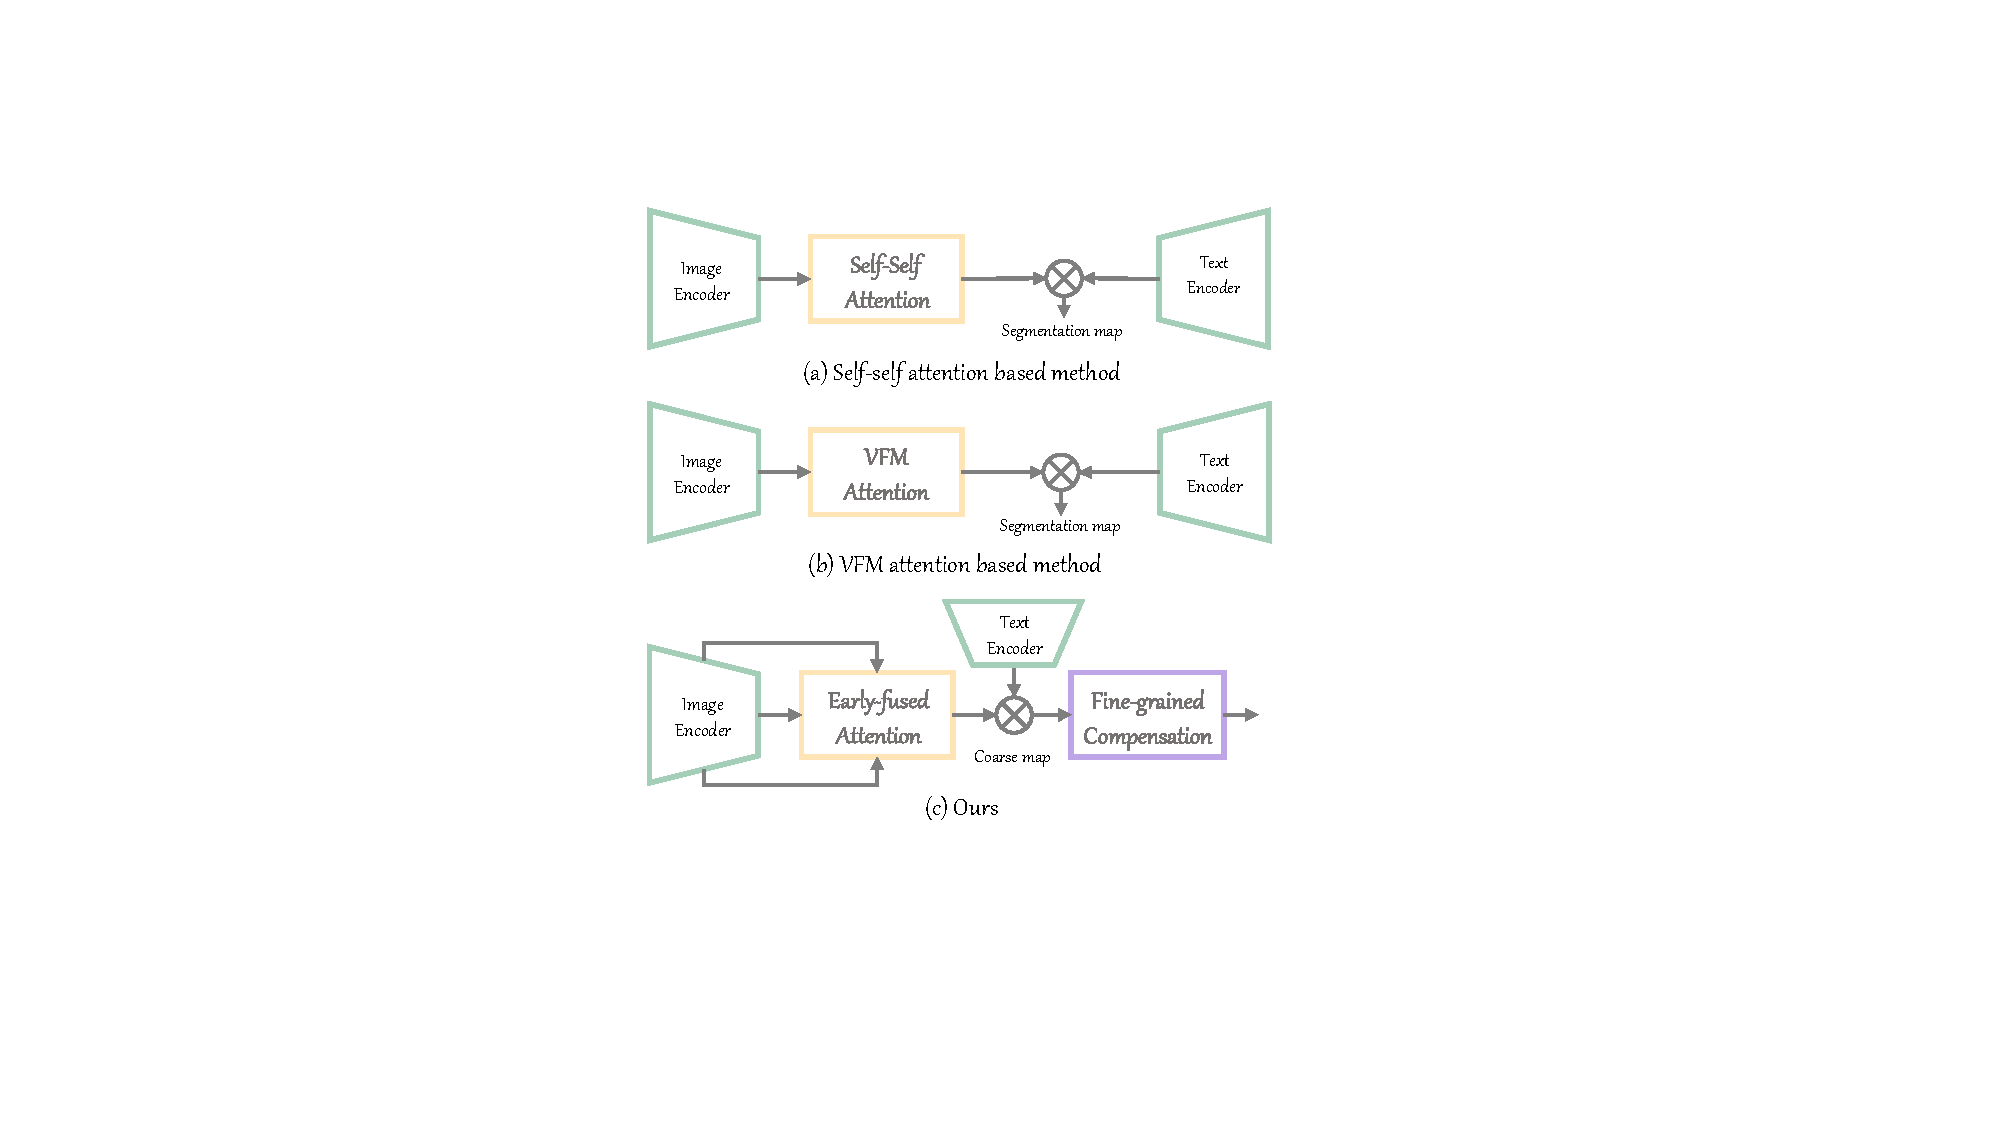
\includegraphics[width=0.9\linewidth]{Fig/fig_CLIPer.pdf}
    \caption{Training-free spatial repair for CLIP-based open-vocabulary segmentation. Self-self attention based methods replace CLIP's original last-layer attention to improve patch coherence, while VFM-attention based methods borrow attention maps from an external vision foundation model. CLIPer instead fuses early-layer CLIP information to form a coarse text-aligned segmentation map and then applies fine-grained compensation to recover local details~\citep{lsunCliperHierarchicallyImproving2025}.}
    \label{fig:open-vocab-cliper}
\end{figure}

Another line of work avoids target training and tries to extract dense localization already present in foundation models. Fig.~\ref{fig:open-vocab-cliper} illustrates the common logic of this route: the language classifier is kept, but the spatial pathway of CLIP is modified or supplemented before text-image similarity is used for pixel prediction. PnP-OVSS uses text-to-image cross-attention, image-text matching gradients, and salience dropout to obtain class masks from off-the-shelf VLMs without pixel-level annotations or finetuning~\citep{luo2024pnpovss}. ITACLIP improves training-free CLIP segmentation through architectural changes, image engineering, and auxiliary text such as definitions or synonyms~\citep{maaydinItaclipBoostingTrainingfree2025}. CLIPer mines early-layer spatial information and then compensates local detail with diffusion-model cues~\citep{lsunCliperHierarchicallyImproving2025}. CorrCLIP further analyzes patch correlations and argues that inter-class correlations impair CLIP's segmentation behavior; it uses SAM to restrict patch interactions and self-supervised features to suppress cross-class noise~\citep{dzhangCorrclipReconstructingPatch2025}. Trident combines CLIP, DINO, and SAM in a training-free splice-then-segment paradigm, using SAM's high-resolution correlations to address CLIP's resolution and receptive-field limitations~\citep{shiyHarnessingVisionFoundation2025}.

In summary, CLIP-based dense alignment is effective because it preserves broad language-defined recognition and requires little task-specific annotation. However, its gains often come from repairing one of three weaknesses: patch features are not sufficiently spatial, text embeddings are not always calibrated to local visual evidence, and high-resolution segmentation stresses CLIP's original input design. This route therefore provides the semantic base for open-vocabulary segmentation, but it is rarely sufficient by itself when precise mask geometry or part-level localization is required.

\subsection{Proposal-then-classification pipelines}

Proposal-then-classification pipelines decouple the spatial and semantic parts of open-vocabulary segmentation. A class-agnostic segmenter first produces candidate masks, and a vision-language classifier then assigns open-vocabulary labels to each mask. This design is appealing because it separates ``where'' from ``what'': the mask generator can specialize in objectness or region boundaries, while the classifier can use text embeddings to recognize categories outside the training vocabulary. It also naturally extends from semantic segmentation to instance and panoptic settings, where masks rather than pixels become the basic prediction units.

OVSeg is a representative two-stage method. Its analysis with oracle masks and oracle classification shows that masked-region classification can be a stronger bottleneck than proposal generation, because masked crops differ substantially from the natural images used to pre-train CLIP~\citep{liang2023ovseg}. Mask-Adapter revisits the same issue from the mask embedding perspective. It shows that direct mask cropping and direct mask pooling can both have limited upper bounds even with ground-truth masks; instead, it extracts semantic activation maps from proposal masks and CLIP features, then constructs more robust mask embeddings with contextual information~\citep{yliMaskadapterDevilMasks2025}. Effective SAM Combination and several SAM-based open-vocabulary methods further use SAM proposals as the spatial substrate, but they still require careful semantic classification and mask filtering~\citep{mleeEffectiveSAMCombination2025,xhanBoostingSegmentAnything2025}.

\begin{figure*}[htbp]
    \centering
    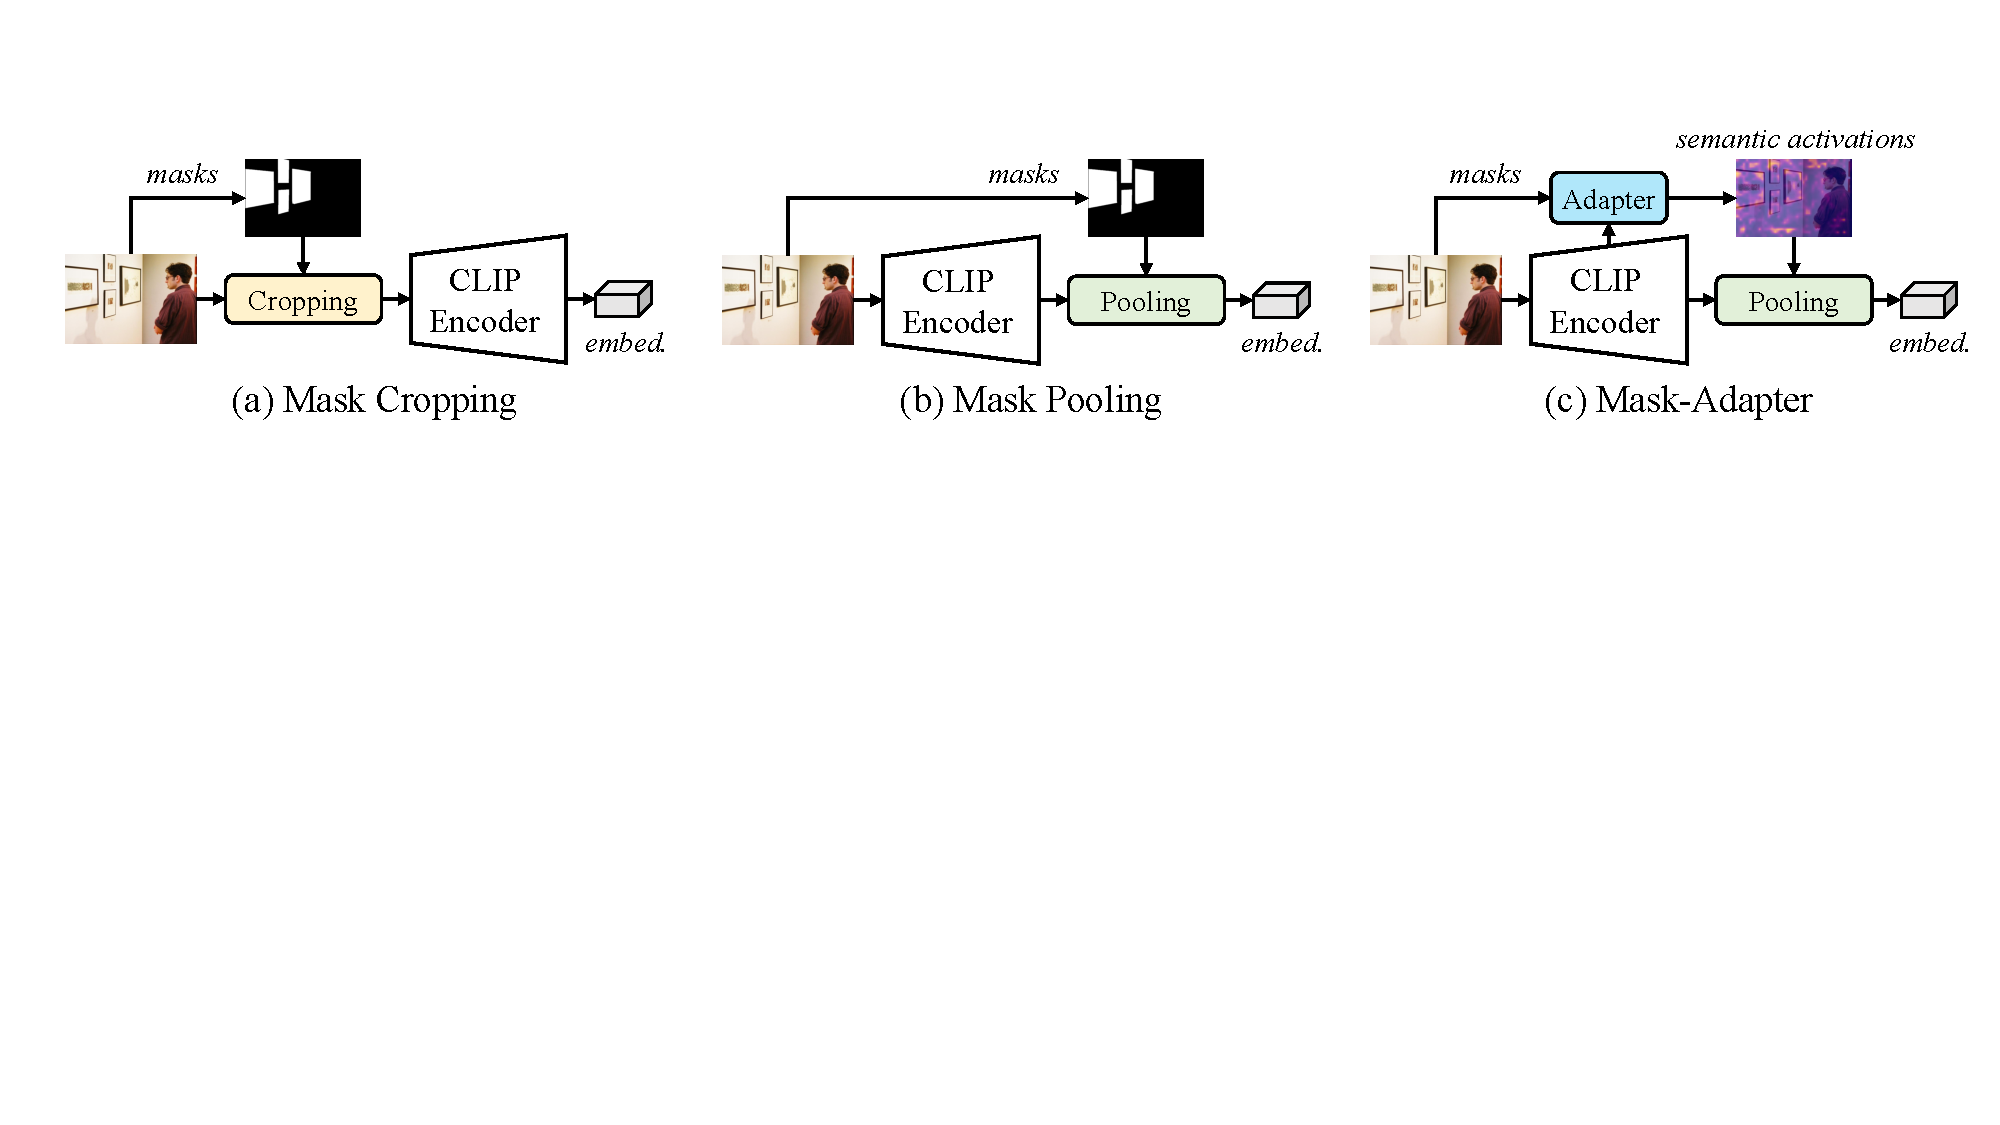
\includegraphics[width=0.98\textwidth]{Fig/fig_MASK.pdf}
    \caption{Mask embedding extraction in proposal-then-classification pipelines. Mask cropping feeds cropped masked regions into CLIP, while mask pooling aggregates CLIP features directly inside proposal masks. Mask-Adapter adds an adapter that converts proposal masks and CLIP features into semantic activation maps before pooling, thereby injecting contextual and mask-aware cues into the final mask embedding~\citep{yliMaskadapterDevilMasks2025}.}
    \label{fig:open-vocab-maskadapter}
\end{figure*}


Fig.~\ref{fig:open-vocab-maskadapter} makes the mask-classification bottleneck explicit. The first two branches rely on the mask itself as the only spatial selector, either before or after CLIP encoding. The adapter branch instead learns where the proposal mask should activate CLIP features for recognition, which explains why high-quality masks and high-quality mask embeddings are separate requirements. Universal segment embedding methods generalize this proposal view. USE builds a data pipeline that automatically curates segment-text pairs at multiple granularities and trains a lightweight segment embedding model, making each mask comparable with arbitrary textual descriptions~\citep{xwangUseUniversalSegment2024}. ReME takes a data-centric, training-free perspective: it constructs a refined reference set of segment-text embeddings from real images and performs simple similarity retrieval during inference~\citep{xxuanReMEDataCentricFramework2025}. These methods show that proposal-level recognition is not just a classifier design problem. The diversity, granularity, and correctness of segment-text data can determine whether a model recognizes object parts, attributes, and contextual labels.




The USE framework in Fig.~\ref{fig:open-vocab-use} also clarifies why segment-level data curation has become a method component: the model learns a reusable embedding space for masks, not just a closed-set classifier for a dataset. The main limitation of proposal pipelines is error coupling. If the proposal generator misses a small object or merges two categories into one mask, the classifier cannot recover the correct dense prediction. If the classifier is poorly calibrated, high-quality masks may still receive wrong labels. If the pipeline uses SAM, DINO, CLIP, diffusion models, and retrieval modules simultaneously, inference cost and reproducibility become difficult to compare. For this reason, proposal-based results should always report the mask generator, proposal budget, classifier backbone, prompt template, and whether the method uses target-domain images or external reference data.

\subsection{Fine-grained semantic and part-level segmentation}

Open-vocabulary segmentation becomes more challenging when the requested labels are not only object categories but also attributes, parts, materials, functional regions, or hierarchical concepts. In classic semantic segmentation, the label set hides many of these distinctions. In open-vocabulary segmentation, the label itself is part of the model interface, so the quality of names and descriptions directly affects both training and evaluation.

Several methods therefore enrich the text or segment side. USE explicitly curates segment-text pairs for objects, parts, and subparts, using MLLM-generated detailed descriptions, grounding models, and mask generators to produce multi-granularity supervision~\citep{xwangUseUniversalSegment2024}. LangHOPS extends this motivation toward language-grounded hierarchical open-vocabulary part segmentation, where part taxonomies and compositional descriptions matter more than flat class names~\citep{ymiaoLanghopsLanguageGrounded2026}. Coconut-PanCap connects panoptic segmentation with grounded captions, indicating that fine-grained visual understanding may require both mask prediction and descriptive generation~\citep{dengCoconutpancapJointPanoptic2026}. Although these works begin to overlap with grounded segmentation, their open-vocabulary relevance is clear: a useful label space is not only larger, but also more precise and structured.

Benchmark-oriented work makes the same point from the evaluation side. RENOVATE shows that many segmentation benchmarks contain class names that are inaccurate, too general, or missing visual context; renovating names can improve both training efficiency and evaluation diagnosis~\citep{hhuangRenovatingNamesOpenvocabulary2024}. FLOSS and related analyses further show that prompt construction, label names, and semantic-space similarity can change the measured performance of open-vocabulary segmentation~\citep{ybenigmimFlossFreeLunch2025,yliuSteppingOutSimilar2025}. These findings caution against interpreting an mIoU gain as purely visual progress. Part of the gain may come from better aligning the textual vocabulary with the visual segments that the benchmark actually contains.

Fine-grained semantic segmentation therefore shifts the question from ``can the model segment unseen classes'' to ``can the model use the right level of language for the right visual region.'' This shift is important for downstream scenarios such as remote sensing, medicine, affordance grounding, and embodied perception, where a label may refer to a functional component, a clinically relevant region, a geospatial structure, or an action affordance rather than a common object category. It also prepares the transition to grounded and reasoning segmentation: once language moves beyond flat class names, the model must understand relations, context, and intent, not only match a word to a mask.

\begin{figure}[htbp]
    \centering
    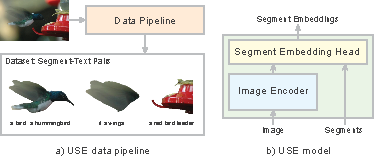
\includegraphics[width=0.98\linewidth]{Fig/fig_USE.pdf}
    \caption{Universal segment embeddings for open-vocabulary segmentation. USE first builds segment-text pairs, such as object, part, and context descriptions associated with masks, and then trains a segment embedding head on top of an image encoder. At inference time, the same image features can be reused with different input segments, producing text-aligned segment embeddings for classification, retrieval, or ranking~\citep{xwangUseUniversalSegment2024}.}
    \label{fig:open-vocab-use}
\end{figure}



\subsection{Efficiency, adaptation, and distillation}

The fourth route studies how to deploy open-vocabulary segmentation under limited supervision, limited compute, or distribution shift. Full finetuning on segmentation labels can improve dense accuracy, but it risks narrowing the open-vocabulary capability inherited from large-scale vision-language pre-training. Training-free methods preserve the original foundation models, but they can be brittle under domain shifts, corruptions, high resolution, or uncommon label vocabularies. Parameter-efficient adaptation, distillation, retrieval, and test-time adaptation therefore occupy the middle ground.

Adapter and prompt-based methods modify a small part of the model while keeping most foundation weights fixed. SAN is an early example of this principle because its side adapter is lightweight and CLIP remains frozen~\citep{xu2023san}. Later work explores parameter-efficient finetuning in hyperspherical spaces, semantic library adaptation, prompt refinement, and LoRA-style retrieval or fusion to adapt CLIP-like representations without full retraining~\citep{zpengParameterefficientFinetuningHyperspherical2025,rqorbaniSemanticLibraryAdaptation2025}. Class-distribution induced attention and feature purification methods similarly try to suppress noisy or outlier features that propagate through dense predictions~\citep{dukangClassDistributioninducedAttention2025,sjinFeaturePurificationMatters2025,qchenTrainingFreeClassPurification2025}. The common goal is to add segmentation-specific structure without destroying the broad semantic space.

Distillation and foundation-model composition provide another practical route. Shinh et al. study open-vocabulary semantic segmentation without semantic labels by leveraging signals from DINO and SAM, showing how vision foundation models can supply dense structure when category labels are scarce~\citep{shinhOpenvocabularySemanticSegmentation2024}. Efficient zero-shot amodal or remote-sensing methods further adapt foundation knowledge to domains where dense annotation is expensive and object appearance differs from natural-image benchmarks~\citep{liuEfficientFoundationModel2025,libExploringEfficientOpenvocabulary2026}. Test-time adaptation addresses a complementary setting: MLMP adapts VLM-based segmentation during inference by combining multi-level visual features and multiple prompt templates, and introduces a benchmark suite with corruptions and real or rendered shifts~\citep{noorimTesttimeAdaptationVisionlanguage2026}. This line is important because a model that performs well on clean VOC or ADE20K may still fail under weather, sensor, domain, or rendering shifts.

Efficiency should be treated as part of the method claim rather than an implementation detail. A training-free system may avoid finetuning but call several large foundation models, run sliding-window inference, generate synthetic visual prompts, or retrieve from a large reference set. A compact adapter may be faster but depend on seen-category training data. A SAM-assisted method may improve boundaries but add proposal generation and filtering cost. Consequently, open-vocabulary segmentation papers should report not only mIoU or AP, but also trainable parameters, inference resolution, foundation modules, prompt budget, target-data usage, and external resources.

\subsection{Summary and discussion}

Several conclusions can be drawn from the methods reviewed above. First, open-vocabulary segmentation is built on a productive but imperfect transfer: image-text foundation models provide flexible semantics, while segmentation demands local, boundary-aware, and well-calibrated dense predictions. Most technical progress can be interpreted as reducing this transfer gap at the pixel, patch, region, or mask level.

Second, mask-centric methods show that spatial priors and semantic classifiers should be evaluated separately. Strong class-agnostic masks do not guarantee correct open-vocabulary labels, and strong CLIP-style recognition does not guarantee complete object masks. This explains why proposal quality, mask embedding extraction, text prompt design, and segment-text data quality all appear as recurring method components.

Third, the benchmark itself is part of the open-vocabulary problem. Class names, synonyms, label granularity, base/novel splits, and prompt templates can change the measured capability. Benchmark-renovation work therefore supports a broader claim of this survey: fair comparison requires a complete reporting protocol, not just a leaderboard number.

Finally, this section clarifies the boundary to the next two method families. Open-vocabulary segmentation answers how a model assigns text-defined categories to dense regions. Promptable and grounded segmentation, reviewed next, asks how masks are controlled and linked to phrases, boxes, points, regions, and generated language. Reasoning segmentation then asks how the target itself is inferred before the mask is produced. The three routes share foundation models, but they test increasingly flexible interfaces: category names, grounded prompts, and reasoning queries.
